% !TEX root =  ../main.tex



In this section we define a probabilistic model that describes the movement of electrons that define an linear topology reactions.
We represent a set of molecules as a set of graphs $\moleculeSet$, with atoms $\Ac$ as vertices and bonds $\Bc$ as edges;
each connected component of the graph defines an individual molecule.
We can associate an ordering over all the atoms in all the molecules in the set using an {\em atom map} number:
an integer label assigned to each non-hydrogen atom in both the reactants and the products which 
both permits easy matching between atoms before and after the reaction, and
%\footnote{In the USPTO dataset, all reactions have been ``atom mapped'', which means that integer labels have been assigned to each non-hydrogen atom in both the reactants and the products.}. 
gives us a consistent way to index particular atoms.
Each atom $v \in \Ac$ includes a set of features, such as its atom type (e.g. carbon, oxygen, \dots); the full list of input atom features can be found in Table 1 of the Appendix.
Input molecules into the model are first put in a Kekul\'e form, a process which makes explicit the location of single and double bonds in aromatic structures;
each bond $b \in \Bc$ is either a single, double, or triple bond.


Given an initial set of reactant molecules $\moleculeSet_0$ and a set of reagent molecules $\moleculeSet_r$, 
our model defines a conditional distribution over a sequence of atoms (which we also refer to as actions) $\electronPath_{0:T} = (a_0, a_1, \ldots, a_T)$,
which fully characterizes the electron path.
This electron path in turn deterministically defines both a final product $\moleculeSet_{T+1}$, 
denoting the outcome of the reaction,
as well as a sequence of intermediate products $\moleculeSet_t$, for $t = 1,\dots,T$,
which correspond to the state of the graph after the first $t$ steps in the subsequence $\electronPath_{0:t} = (a_0, \dots, a_t)$ are applied to the initial $\moleculeSet_0$. We also define a stopping sequence $\mathcal{S}_t = (s_0, \ldots, s_T)$ which indicates if the reaction should stop (i.e, $s_t\!=\!1$ if the reaction should stop and is $0$ otherwise). 

We propose to learn a distribution $p_\theta( \electronPath_{0:T} \mid \moleculeSet_0, \moleculeSet_r)$ over electron movements. 
We first detail the generative process %(i.e., the forward pass) 
that specifies $p_\theta$, before describing how to train the model's parameters.


\subsection{Generative process}

%The distribution over electron paths can be factorized as follows:
%%\begin{align}
%%p_\theta(\electronPath \mid \moleculeSet_0) = p_\theta(s_{0}' \mid \moleculeSet_0) p_\theta(a_{0} \mid \moleculeSet_0) \prod_{t=1}^{T-1} \left( p_\theta(a_{t} \mid a_{t-1}, \Mc_{t-1} ) p_\theta(s_{0}' \mid \moleculeSet_0) \right) p_\theta(a_{T} \mid a_{T}, \Mc_{T-1} ) p_\theta(s_{T} \mid \moleculeSet_T) \nonumber
%%\end{align}
%
%\begin{align*}
%p(\electronPath_{0:T} \mid \initialAndReactants) = &
% \quad 
% p(s_0' \mid \initialAndReactants)
% p(a_0 \mid \initialAndReactants)
% \prod_{t=1}^{T} \Big[ 
% 	p(s_t' \mid \initialAndReactants, \electronPath_{0:t-1})
% 	p(a_t \mid \initialAndReactants, \electronPath_{0:t-1} ) 
% \Big] \\
% & \times p(s_{T+1} \mid  \initialAndReactants, \electronPath_{0:T} )
%\end{align*}

%\improvement[]{this part a bit messy}
%Where $p(s_{t})$ is the probability of stopping the path before picking the $t^{\text{th}}$ action, $p(s_{t}')$ of continuing.


\begin{figure*}
\centering
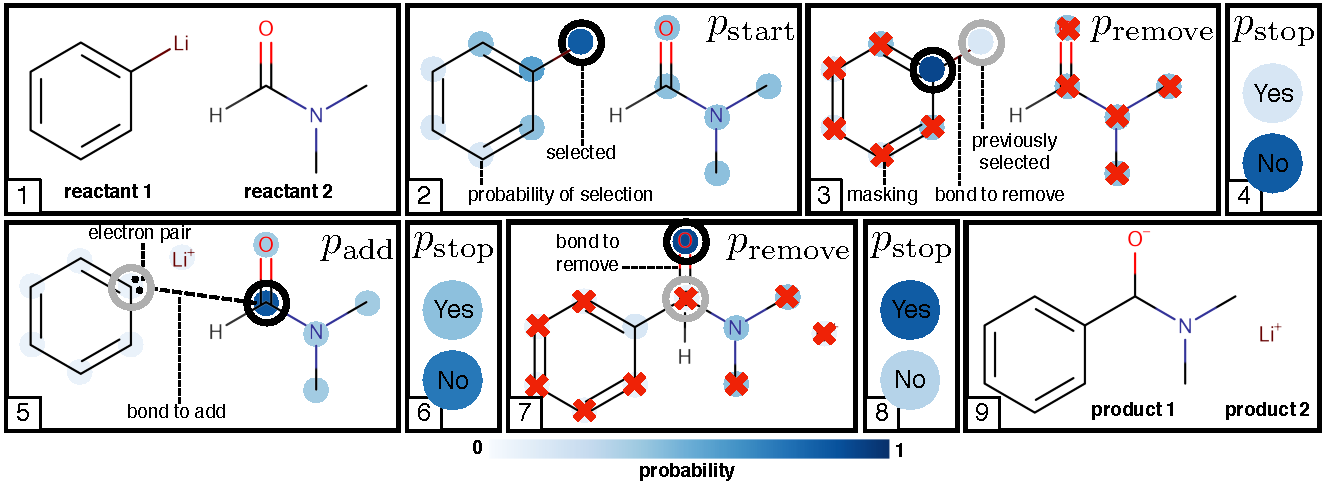
\includegraphics[width=\textwidth]{reaction_model_blue}
\caption{
 This figure shows the sequence of actions in transforming the reactants in box 1 to the products in box 9.
 The sequence of actions will result in a sequence of pairs of atoms, between which bonds will alternately be removed and created, creating a series of intermediate products. 
At each step the model sees the current intermediate product graph (shown in the boxes) as well as the previous action, if applicable, shown by the grey circle. It uses this to decide on the next action.
We represent the characteristic probabilities the model may have over these next actions as colored circles over each atom.
Some actions are disallowed on certain steps, for instance you cannot remove a bond that does not exist; these blocked actions are shown as red crosses.
}
\label{fig:reaction_model}
\end{figure*}




First note that since our reactions are a single path of electrons through the reactants then, at any point, the next step in the path depends only on (i) the intermediate molecule formed by the action path up to that point, (ii) the previous action taken (indicating where the free pair of electrons are) and (iii) the point of time through the path, indicating whether we are on an add or remove bond step. 
%In practice we assume that the probability of an action depends only on (i) the intermediate molecule formed by the action path up to that point, (ii) the previous action taken (indicating where the free pair of electrons are) and (iii) the point of time through the path, indicating whether we are on an add or remove bond step. 
We make the simplifying assumption that the stop probability and the actions after the initial action $a_0$ do not depend on the reagents. This leads to a parameterized model with dependency structure:
\begin{align}
\label{eq:jointprob}
p_\theta(\electronPath_{0:T} \mid \moleculeSet_0, \moleculeSet_r) 
&=
	p_\theta(s'_0 \mid \moleculeSet_0)
	p_\theta(a_0 \mid \moleculeSet_0, \moleculeSet_r)\\ \nonumber &\quad \times
	\left[\prod_{t=1}^{T}
		p_\theta(s_{t}' \mid \moleculeSet_{t})
		p_\theta(a_t \mid \moleculeSet_{t}, a_{t-1}, t)
	\right]
	p_\theta(s_{T+1} \mid \moleculeSet_{T+1})
	,
\end{align}
where we have defined $p_\theta(s'_t \mid \moleculeSet_t) \equiv 1 - p_\theta(s_t \mid \moleculeSet_t)$ to be the probability of {\em continuing} a reaction given the current molecule set $\moleculeSet_t$.
The other terms include $p_\theta(a_0 \mid \initialAndReactants)$, the probability of the initial state $a_0$ given the reactants and reagents; 
the conditional probability $p_\theta(a_t \mid  \moleculeSet_t, a_{t-1}, t)$ 
%\todo[]{maybe somehow refer to "bond type" instead of $t$?} 
of next state $a_t$ given the intermediate products $\moleculeSet_t$ for $t > 0$;
and the probability $p_\theta(s_t \mid \moleculeSet_t)$ that the reaction terminates with final product $\moleculeSet_{t}$.

%
%
%%% THIS IS THE PREVIOUS VERSION:
%\begin{align*}
%p_\theta(\electronPath_{0:T} \mid \moleculeSet_0, \moleculeSet_r) = &
% \quad \continueProb{0}{0}
%       p(a_0 \mid \moleculeSet_0, \moleculeSet_r)
%       p(a_1 \mid \moleculeSet_0, a_0) \\
%       & \times \prod_{t=2}^{T} \Big[
%              \continueProb{t}{\electronPath_{0:t-1}}
%              \actionProb{t}
%       \Big] \\
%       & \times p(s_{T+1} \mid \moleculeSet_{\electronPath_{0:T}})
%\end{align*}
%

It is possible to stop prior to selecting a first atom $a_0$, indicating that no reaction would take place.
However, we restrict our model to not stop $t\!=\!1$, as it is necessary to pick up a complete electron pair. 
Given any particular selected atom $a_t$ which extends the reaction path, we can deterministically update the previous molecular graph $\moleculeSet_{t}$ to produce the next set of (intermediate) products $\moleculeSet_{t+1}$.

Given our reaction assumptions, then, as stated earlier, there are two types of electron movements that alternate: 
(i) movement that \emph{removes an existing bond}, and 
(ii) movement that \emph{adds a new bond}. 
%We can generalize assumption 3 by defining that atoms with free electrons have a self-bond. 
We define atoms with free electrons as having a self-bond.
%\todo[]{...or implicit hydrogens?}
Thus, all reactions start by first selecting an atom, removing a bond (between two different atoms, or a self-bond), and then alternately adding and removing bonds;
we can determine whether a particular step is an add step or remove step by inspecting $t$.
Note that $\moleculeSet_1 = \moleculeSet_0$, as the initial action of selecting $a_0$ does not form or remove any bonds.
%\todo{maybe put this somewhere else}.
Figure~\ref{fig:reaction_model} presents a simple example reaction which demonstrates all the critical features of the model;
the subfigures show the sequence of intermediate products and the distributions over actions.
%The first subfigure shows two reactants, which we assume will react (i.e.\ $s_0' = 1$).
%Subsequent subfigures show the network picking an initial atom to begin the electron path,
%and then iteratively selecting atoms for removing and adding bonds, potentially stopping after each action.
%Masking at each add and remove step can reduce the total number of possibilities: 
%for example, it is not possible to remove a bond which does not exist in the graph $\moleculeSet_t$.
%\todo[]{walk through figure. do we want to that HERE, or in the caption? or elsewhere?}


Each of the conditional probabilities in Eq.~\eqref{eq:jointprob} are parameterized by neural networks:
for each stage the network takes the current intermediate graphs, 
the previous action, and the reagents if relevant, 
and computes a probability distribution over next possible actions (i.e., selecting a particular atom, or stopping).
The structure of these networks is described in the following section.
% and more detailed information on the architectures is given in the supplementary material.

\subsection{Computing atom and molecule features}


We are left now with defining the functional form of our conditional distributions for continuing $p_\theta(s'_t \mid \moleculeSet_t)$, picking the initial action $p_\theta(a_0 \mid \initialAndReactants)$, and picking subsequent actions $p_\theta(a_t \mid \moleculeSet_t, a_{t-1}, t)$.
However, before describing these modules we need to describe how we compute node embeddings and graph embeddings, as these  are  essential to each.
Full architectural details (e.g.\ number of layers and hidden units) 
and training settings are deferred to the Appendix.

Node embeddings are representations of all the atoms in all the molecules present in $\moleculeSet_t$.
 We denote them by the matrix $\nodeEmbeddings{\moleculeSet_t} \subseteq \mathbb{R}^{|\Ac|\times d}$.
Each row contains a $d$-dimensional embedding of an atom. 
A natural ordering for the rows are the atom-map numbers assigned to each atom.
We define the function $\fEmbed$ to map a set of graphs representing each molecule to these node embeddings.
In general $\fEmbed$ could be any graph model that uses the graph structure of $\Mc_t$ to get graph-isomorphic node features, usually via message-passing techniques \citep{gilmer2017neural};
we choose to use gated graph neural network (GGNN) message functions \citep{li2016gated}.

It is also useful to be able to calculate graph embeddings $\graphEmbeddings$, which are vectors that represent groups of nodes belonging to one or more graphs; i.e.\ an entire molecule or set of molecules.
 We define the function that maps node features belonging to each atom to their graph embedding by $\fEmbedGraphs$.
These are similar to the readout functions used for regressing on graphs detailed in \citep[Eq. 3]{gilmer2017neural} and the graph embeddings described in \citet[\S B.1]{li2018learning}. 
Specifically, $\fEmbedGraphs$ consists of three functions, $\fui$, $\fuj$ and $\fuk$, which could be any MLP but in practice we find that linear functions suffice. % use linear layers for.
They are used to form the graph embedding, $\graphEmbeddings$, in the following way:
\begin{align}
%	\graphEmbeddings = \fuk\big(\sum_{v \in \Ac'} \left[ \mbox{sigmoid}(\fui(\Hb_{\Ac,v})) \cdot \fuj(\Hb_{\Ac,v}) \right]\big).
	\graphEmbeddings = \fEmbedGraphs(\nodeEmbeddings{\moleculeSet_t}) = \fuk\left(\sum_{v \in \Ac'} \sigma\left(\fui(\nodeEmbeddings{\moleculeSet_t,v})\right) \fuj(\nodeEmbeddings{\moleculeSet_t, v})\right).
	\label{eq:graph-embedding}
\end{align}
We can break this down into two stages.
In stage (i), similar to \citet[\S B.1]{li2018learning} we form an embedding of one or more molecules (with vertices $\Ac'$), by performing a gated sum over the node features.
In this manner the function $\fui$ is used to decide how much that node should contribute towards the embedding,
 and $\fuj$ projects the node embedding up to a higher dimensional space; following \citet[\S B.1]{li2018learning}, we choose this to be double the dimension of the node features.
Having formed this embedding of the graphs, we project this down to a lower dimensional space in stage (ii), which is done by the function $\fuk$. 
%Again we use a single linear layer for this function. % already said this above


\subsection{Computing our probabilities over actions}

Having described how we compute node and graph embeddings, we are now ready to define each of our parameterized distributions over actions.
The simplest of these is $p_\theta(s'_t \mid \moleculeSet_t)$, which is the probability of continuing given the set of intermediate products at time $t$. 
This probability is computed as a graph embedding $\fEmbedGraphs_{\textrm{stop}}$,
whose functional form is defined by Eq.~\eqref{eq:graph-embedding}, which projects down to a single dimension followed by a sigmoid function
\begin{align}
%$
p_\theta(s'_t \mid \moleculeSet_t) = \sigma(\fEmbedGraphs_{\textrm{stop}}(\nodeEmbeddings{\moleculeSet_t})).
%$
\end{align}
%
%This leaves us with describing the form of the initial action, $p_\theta(a_0 \mid \initialAndReactants)$, and picking subsequent actions, $p_\theta(a_t \mid a_{t-1} \moleculeSet_t, t)$, modules.
% The second of these can be broken down into two parameterized functions
Each of the three parameterized conditional probability distributions for the {\em start}, {\em add} and {\em remove} steps have similar forms, each defining a probability vector over actions.
The transition distribution $p_\theta(a_t \mid  \moleculeSet_t, a_{t-1}, t)$ 
which selects the next atom in the sequence $\electronPath$
can be split into two distributions depending on the parity of $t$:
the remove bond step distribution $p_\theta^\textrm{remove}(a_t \mid  \moleculeSet_t, a_{t-1})$ is taken when $t$ is odd, 
and the add bond step $p_\theta^\textrm{add}(a_t \mid \moleculeSet_t, a_{t-1})$ is taken when $t$ is even. 

These three modules each have the same overall functional form
\begin{align}
\actionLogits &= f(\nodeEmbeddings{\moleculeSet_t}, \contextVect), \\
p_\theta(a_t \mid \cdots) &\propto \bm{\beta} \odot \mbox{softmax}(\bm{\actionLogits})
\end{align}
where $f$ is one of the networks $\fInitial, \fAdd$, or $\fRemove$; 
$\contextVect$ is a context vector, and $\bm{\beta}$ is a binary mask.

Each of the three actions has a different context and mask.
The add step $p_\theta^\textrm{add}(a_t \mid \moleculeSet_t, a_{t-1})$ and remove step $p_\theta^\textrm{remove}(a_t \mid \moleculeSet_t, a_{t-1})$,
 have as context the node embedding of the atom selected at the previous step, $\contextVect_{a_{t-1}} = \nodeEmbeddings{\moleculeSet_t, a_{t-1}}$. 
For the initial step, this context vector $\contextVect_\mathrm{reagent}$ is an embedding of all the reagents present, computed %by summing graph embeddings for reagent, each computed using
by a graph embedding function $\fEmbedGraphs_\mathrm{reagent}$.
%\todo[]{I think this is implicitly summing over all reagents, since we aren't restricting anywhere to only summing over atoms in a single connected component...?}
When computing the output probabilities,
we use the binary vector $\bm{\beta}$ to mask out specific actions known to be impossible.
%When computing The $\bm{\beta}$ term is a binary vector, that allows us to mask out specific actions. 
The value of this differs for the {\em start}, {\em add} and {\em remove} steps;
for the initial step any action can be picked, so this is one everywhere.
For the remove step, $\bm{\beta}_\mathrm{remove}$ masks out (i.e.\ is set to zero for) any bonds that do not currently exist and thus cannot be removed (noting though that self-bonds are permitted in the first remove step).
For the add step, $\bm{\beta}_\textrm{add}$ only masks out the previous action, preventing an atom from bonding with itself.


% Each of these modules begin by computing  a single value for each node, so for the initial step we have 
% $\actionLogits_{\textrm{start}, v} = \fum^\textrm{start}(\nodeEmbeddings{\moleculeSet_t,v}, \contextVect)$ where $\fum$ is a NN and $\contextVect$ is a context vector. 
% The expressions are similar for the add and remove modules, however with different NNs used for the respective $\fum$ functions.
% Moreover, they also differ in the context vectors $\contextVect$ which they use:
% the add step $p_\theta^\textrm{add}(a_t \mid \moleculeSet_t, t)$ and remove step $p_\theta^\textrm{remove}(a_t \mid \moleculeSet_t, t)$,
% have as context the node embedding of the atom selected at the previous step, $\contextVect_{a_{t-1}} = \nodeEmbeddings{\moleculeSet_t, a_{t-1}}$. 
%For the initial step, this context vector $\contextVect_{r}$ is an embedding of all the reagents present, computed %by summing graph embeddings for reagent, each computed using
%by a graph embedding function $\fEmbedGraphs_r$.
%\todo[]{I think this is implicitly summing over all reagents, since we aren't restricting anywhere to only summing over atoms in a single connected component...?}
%
%Finally, each of the modules compute the probability vector over actions. 
%So again starting with the initial step we have 
%$p_\theta(a_0 \mid \initialAndReactants) \propto \bm{\beta_\textrm{start}} \odot \mbox{softmax}(\bm{\actionLogits_{\textrm{start}}})$, 
%with again similar terms for the add and remove steps.  
%The $\bm{\beta}$ term is a binary vector, that allows us to mask out specific actions. The value of this differs for the {\em start}, {\em add} and {\em remove} steps. 
%For the initial step any action (or atom) can be picked and so this is 1 everywhere. For the remove step, $\bm{\beta_\textrm{remove}}$ masks out bonds that do not currently exist (although self bonds are allowed in the first step).
%For the add step, $\bm{\beta_\textrm{add}}$ only masks out the previous action.
%

\paragraph{Training}
We can learn the parameters $\theta$ of all the parameterized functions, by maximizing the likelihood of the true path $\log p_\theta(\electronPath_{0:T} \mid \moleculeSet_0, \moleculeSet_r)$.
%\begin{align*}
%%  \min_{\fModules}
%\min_{\theta}
%    & - \log \continueProb{0}{0} - \log p(a_0 \mid \moleculeSet_0, \moleculeSet_r)  - \log p(a_1 \mid \moleculeSet_0, a^*_0) \\
%	& - \sum_{t=2}^{T} \log \Big[ \continueProb{t}{\electronPath_{0:t-1}^*} \actionProb[*]{t} \Big] \\
%    & - \log p(s_{T+1} \mid \moleculeSet_{\electronPath_{0:T}^*})
%\end{align*}
This is evaluated by using a known true electron path $a_t^\star$ and intermediate products $\moleculeSet_t^\star$ extracted from training data,
rather than on simulated values. 
This allows us to train on all stages of the reaction at once, given electron path data.
We train our models using ADAM \citep{kingma2014adam} and an initial learning rate of $10^{-4}$,
with minibatch sizes of one, although these can consist of multiple intermediate graphs.

\paragraph{Prediction}
Once trained, we can use our model to sample chemically-valid paths given an input set of reactants $\moleculeSet_0$ and reagents $\moleculeSet_r$, 
simply by simulating from the conditional distributions until sampling a stop value $s_t$.
We instead would like to find a ranked list of the top-$K$ predicted paths, and do so using a modified beam search,
in which we roll out a beam of width $K$ until a maximum path length $T^\mathrm{max}$,
while recording all paths which have terminated.
This search procedure is described in detail in Algorithm 1 in the Appendix.



